
\chapter{Software Architektur}
\section{Anforderungen}
\label{sec:Anforderungen} 
%Christoph

Im Folgenden sollen die Anforderungen an die Studienarbeit festgelegt werden. \newline
Ein Hauptbestandteil der Arbeit besteht darin, ein Vorgängerprojekt mit einer AR.Drone 2.0 in das ROS Framework zu portieren.
Dies beinhaltet eine Modularisierung der Projektbestandteile in ROS Nodes. Ziel soll sein, den Quadrocopter mit Hilfe einer Kinect und Gestenerkennung steuern zu können. Anzumerken ist, dass ROS nur unter UNIX basierten Betriebssystemen läuft und das bestehende Projekt Libraries verwendet, welche nur unter Windows verfügbar sind. \newline
Eine weitere Vorgabe besteht darin, dass man neben der realen Drohne jegliche Funktionalität auch in einer Simulation laufen soll. \newline
Somit kann man für Präsentationen, in denen der Flug einer Drohne nicht möglich ist, den Quadrocopter in einer frei gestaltbaren simulierten Umgebung fliegen lassen. \newline
Ein weiterer Bestandteil dieser Arbeit besteht darin, Ansätze und Limitationen der Implementierung eines Assistenzsystems zu testen und zu bewerten. Dafür soll ein externes Projekt, zur Gewinnung von Tiefenbildern aus einer monokularen Kamera, in die Projektumgebung integriert werden. Hierbei soll es wiederum möglich sein, dass die Videostream sowohl von der realen, als auch von der simulierten Drohne gesendet werden kann. \newline
Es soll dabei ermittelt werden, ob die Nutzung der Software für den Anwendungszweck praktikabel und sinnvoll ist.

%hier weitermachen, wenn man weiß wie weit wir tatsächlich kommen #wahrscheinlichsindwirzublöd #forschung>implementierung

%	-> Wände / Türen erkennen
%	-> aktives eingreifen der Drohne in das Geschehen -> Kollisionsvermeidung


\section{Überblick}
\label{Überblick}

\section{Implementation}
\label{Implementation}

\newpage


\subsection{SVO}
\subsection{REMODE}
\subsection{Kamerakalibrierung}
Ein Grundproblem der Bildverarbeitung ist die Verzerrung des Bildes. Da aus eingehenden Bildern Features erkannt werden sollen und aus diesen darüber hinaus Abstände berechnet werden, ist es essentiell, dass die Kamera richtig kalibriert ist. \newline
Hierbei unterstützt SVO drei Kamera Modelle: ATAN, Pinhole und Ocam. \cite{svo_cameracalibration} \newline
Das ATAN Model basiert auf dem \textit{Field of View \emph{(FOV)}} Verzerrungsmodell. 




\subsection{Featureerkennung}
\subsection{Kinect}
%Max
\subsection{Architektur/Aufbau}
%Beide
\subsection{Die einzelnen ROS Nodes}
%Beide


%\begin{figure}[ht]
%	\centering
%	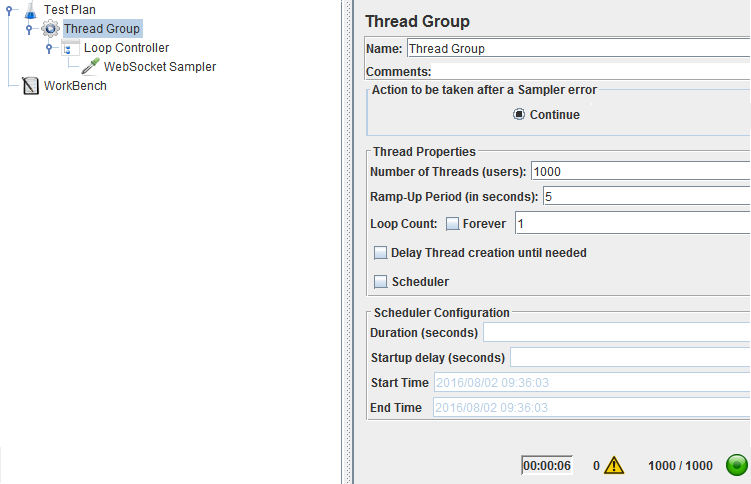
\includegraphics[scale=0.7]{Bilder/jMeterReal.png}
%	\caption[Testing with jMeter]{jMeter testing}
% 	\label{fig:testing}
%\end{figure}


